\chapter{Evaluation}
The following chapter presents the results of the experiments carried out with the \gls{icds}.
Evaluation has been done in different areas to give a complete impression of how the \gls{icds} performs.
In the first section some general findings will be described that affect overall performance.
Afterwards the test environment and setup of the IMSI catcher is discussed.
The last two sections evaluate the \gls{icds} against a configured catcher.
At first the individual rules are tested, then the two attacks described in the theory section were conducted.

\section{Performance Evaluation}
In order to evaluate general performance it has to be considered that the \gls{icds} can be deployed in different environments.
To reflect different compositions and densities of base stations from different areas, four distinct data sets will be used for the experiments in this section.
The data sets have been taken in areas surrounding the city of Freiburg.
For each area three scans were made on a fixed position and the duration was averaged.
Table \ref{tab:key_data} shows some of the data sets' key values.
\begin{table}
\centering
\begin{tabular}{llrr}
\toprule
Name					&Description					&Number of BTS	&Duration\\
\midrule
\texttt{cdb}			&CBD around the area of			&54				&6:13\,m	\\
						&Bertoldsbrunnen				&				&			\\
\texttt{airport}		&Airport and university area	&68				&6:25\,m	\\
						&around Georges K\"ohler Allee	&				&			\\
\texttt{ind\_park}		&Industrial park Haid in 		&53				&4:52\,m	\\
						&Freiburg West,  Hausener Weg	&				&			\\
\texttt{house\_area}	&Housing area at the rim of 	&22				&3:59\,m	\\
						&Freiburg Z\"ahringen, Thuner Weg	&				&			\\
\bottomrule
\end{tabular}
\caption{Key values of the data sets used for performance tests.}
\label{tab:key_data}
\end{table}

Apart from nodes of the four German \gls{gsm} providers E-Plus, T-Mobile, Vodafone and O2, nodes from the Deutsche Bahn also occur in these scans.
These nodes form a private network used for internal communications by the Deutsche Bahn.
They are identified by their broadcast name \emph{DB Systel GSM-R} and their frequency which is a in a range registered to the Deutsche Bahn.
Since the distribution of these nodes is very sparse, only one node can be found in each scan. 
They yield a false positive for no neighbouring nodes can be discovered.
These nodes are not relevant to subscribers because they are not able to connect to them.
Therefore they will be ignored and factored out for the remainder of this evaluation.

\subsection{Scan Duration}
\begin{figure}
\centering
\begin{tikzpicture}
\begin{axis}[
	width=\textwidth,
	height=0.3\textheight,
	xlabel=Total BTSs, 
	ylabel=Scan duration in s,
	xticklabel style={/pgf/number format/1000 sep=}
	]
	\addplot [mark=*, blue, only marks] plot coordinates {
		(68, 385)
		(54, 373)
		(53, 292)
		(22, 239)
	};
\end{axis}
\end{tikzpicture}
\caption{Scan durations for the sample data sets.}
\label{fig:durations}
\end{figure}
Table \ref{tab:key_data} shows that the time needed for a sweep scan in the Freiburg area can differ by large amounts depending on how many base stations have been scanned.
Generally said it takes longer the more dense the base station distribution is in the area.
This is however not the only factor, as Figure \ref{fig:durations} visualises.
If the scan duration would only depend on the number of base stations scanned, a linear growth could be expected.

This is however not the case as the plot shows.
A bad reception means that a lot of \gls{bcch} frames are rendered unusable and have to be retransmitted.
Therefore it takes significantly longer to gather all System Information Messages for a single \gls{bts} that has a bad reception.
Looking at the overall reception in the datasets shows that no base stations in the \texttt{cbd} dataset had a reception of below -95\,dB.
In the three other datasets stations with reception levels of below -100\,dB can be found.
Overall reception was worst in the \texttt{airport} and \texttt{cbd} datasets which explains the large jump in time although only one more base station has been scanned between the \texttt{ind\_park} and \texttt{cbd} datasets.

Re-evaluation of a base station based on its own parameters thus occurs only every seven minutes in the worst scenario we experienced.
This is an inherent problem to the approach of scanning and updating all base stations and not only monitoring a subset belonging to a single provider.
If an IMSI catcher replaces a base station directly after it was scanned, it could take up to seven minutes until it is discovered.
To lessen this threat, if the \gls{icds} is used in \emph{User Mode}, the base station with the strongest reception is scanned again with a PCH scan, to eliminate the possibility of having been taken over and not being detected.

\subsection{Cell ID Databases}
The usefulness of the Cell ID Rule is subject to the completeness of the database that is used.
That is even more so since a database with a low coverage will yield false positives, \eg legitimate base stations will be evaluated as being IMSI catchers because they are not found in the database.

The coverage for the OpenCellID database and the Google Mobile Maps service evaluated against the data sets can be seen in Table \ref{tab:coverage}.
\begin{table}
\centering
\begin{tabular}{lrrcrrcrrcrr}
\toprule
& \multicolumn{2}{c}{\texttt{cdb}} &\phantom{a}& \multicolumn{2}{c}{\texttt{airport}} &\phantom{a} & \multicolumn{2}{c}{\texttt{ind\_park}}&\phantom{a} & \multicolumn{2}{c}{\texttt{house\_area}}\\
\cmidrule{2-3} \cmidrule{5-6} \cmidrule{8-9} \cmidrule{11-12}
&Cov.&Time&	&Cov.&Time&	&Cov.&Time&	&Cov.&Time\\
\midrule
Google&		1.00&5&	&0.99&8&	&1.00&5&	&1.00&2\\
OCID&		0.57&51&	&0.58&68&	&0.58&55&	&0.41&19\\
\bottomrule
\end{tabular}
\caption{Coverage for Google Mobile Maps and OpenCellID on the data sets with the time needed in seconds for fetching the information.}
\label{tab:coverage}
\end{table}
Google Mobile Maps service scored a complete coverage on all the data sets while OpenCellID could cover about half the nodes in the different sets.
The Ericson and combain databases could not be evaluated since it was not possible to obtain an API key without handing out credit card details for billing.
The reason the Google service had only a 99\% coverage on the \texttt{airport} data set is that base station that has not been found was the one operated by the Chair of Communication Systems, therefore it can be factored out.
The OpenCellID database is not a good source of information for this project as is shown by its coverage scores.
Both services also show a large difference in response time.
The time needed to do a single lookup could take up to several seconds while a single lookup on the Google service presented a result almost instantly.
This is most probably due to the fact that Google's server infrastructure is strongly optimised for tasks like this.
The times also show that if the \gls{icds} would be connected to the internet, the lookups on Google's database could also be done during the course of a sweep scan since they do not impose a large time overhead per base station.

However it must be said that these two services are intended for localisation and thus do not have the demand to yield a complete coverage of all the base stations in the area.
Therefore it must be kept in mind when using this rule for analysis that false positives might still be brought forth.
What can be said though is that a base station that has been found may only be subject to a type of attack that replaces an existing base station and can thus be investigated more specifically on that ground.

\subsection{PCH Scans}
In order to establish a baseline on what to expect from the \gls{pch} scans additional measurements have been done.
Table \ref{tab:pagings} shows scans that have been done in the different areas.
In each area the cell with the strongest reception for each provider was chosen as a representative for the respective provider.
The duration of each scan was set to 60 seconds, while the values in the table have been averaged for 10 seconds since this is the unit the \gls{icds} is using.

A comparison of the results suggests that different providers also have different policies when to page.
Vodafone has about six times the paging rate of other providers.
This can be explained by further examining the Vodafone network structure.
Another scan showed that for other providers the Paging Messages were addressed to between 70 and 120 different \glspl{tmsi} whereas for Vodafone between 600 and 700 different \glspl{tmsi} were found.
The large difference in \glspl{tmsi} is due to the fact that Vodafone's \glspl{la} are larger than the \glspl{la} other providers use.
For the Freiburg area two different \glspl{lac} were found for each of the providers E-Plus, T-Mobile and O$_2$ while for Vodafone only one \gls{lac} was found.
These facts were also checked against the OpenCellID database which yielded the same results for \glspl{lac} used in the Freiburg area.
All this gives some insights into the paging policy that Vodafone might have.
If the network is looking for a subscriber the last known \gls{la} for this subscriber is paged rather than starting with the last known cell and expanding the paging radius. 
Since the area covered by a single \gls{la} is very large, a lot of subscribers are registered for a single area.
This theory would also be consistent with the face that despite of the large number of Paging Messages only an average number of \glspl{ia} were caught which are restricted to the serving cell.

Another scan was also done on the IMSI catcher.
No Paging Messages or \glspl{ia} were detected although a \gls{ms} was connected to it.
This was to be expected as formerly discussed in Section \ref{sec:paging} because the IMSI catcher is not actually part of the providers network and thus cannot receive and forward Paging Messages.

\begin{table}
\centering
\begin{tabular}{lrrcrrcrrcrr}
\toprule
& \multicolumn{2}{c}{\texttt{house\_area}} &\phantom{a}& \multicolumn{2}{c}{\texttt{cbd}} &\phantom{a} & \multicolumn{2}{c}{\texttt{airport}}&\phantom{a} & \multicolumn{2}{c}{\texttt{ind\_area}}\\
\cmidrule{2-3} \cmidrule{5-6} \cmidrule{8-9} \cmidrule{11-12}
&PMs.&IAs&	&PMs. &IAs.&	&PMs.&IAs.&&PMs.&IAs\\
\midrule
T-Mobile&		89&3&	&75&3&	&109&4&&72&1\\
E-Plus&		119&1&	&67&2&	&70&1&&65&0\\
Vodafone&		776&6&	&720&5&	&712&6&&743&2\\
O$_{2}$&		117&9&	&106&16&	&94&11&&95&7\\
\bottomrule
\end{tabular}
\caption{Number of Paging Messages and Immediate Assignments (per 10 seconds) for the four German providers at different locations.}
\label{tab:pagings}
\end{table}

\section{IMSI Catcher Detection}
Before using an IMSI catcher for testing purpose or a launching an OpenBTS base station it should be ensured that licenses for the specific frequencies that are used, have been obtained.
This way it can be ensured that the operation does not interfere with regular radio communication.
In case of our experiments we always used \gls{arfcn} 877 and broadcasted '23' as provider name.
The university has acquired a license for this frequency and since the provider identification differs from the four common providers' \glspl{mnc} we do not lure mobile subscribers into connecting to the catcher.

\subsection{Open Source IMSI Catcher}
Some of the rules cannot be tested without an active IMSI catcher.
For this purpose the Open Source IMSI Catcher \cite{dennis} is used.

This project prototypes an IMSI catcher using only open source systems and freely available hardware so it can basically be used and built by anybody.
On the hardware side a computer running a Linux operating system is used, as well as the \gls{usrp} as the radio transmitter.
The \gls{usrp} allows the signal processing for radio transmissions to be done in software, therefore it can be used for a multitude of purposes and protocols.
Some hardware modifications have to be done to the device to empower it to send and receive data on the frequency bands used for \gls{gsm} communication.
An external clock needs to be used since \gls{gsm} operations are very time critical.
Figure \ref{fig:setup} shows the Open Source IMSI Catcher and the \gls{icds} side by side.

On the software side GNU Radio\footnote{GNU Radio Project Wiki, \url{http://gnuradio.org/redmine/projects/gnuradio/wiki} [Online; Accessed 05.2012]}, OpenBTS\footnote{OpenBTS Project Wiki, \url{http://wush.net/trac/rangepublic} [Online; Accessed 05.2012]} and Asterisk\footnote{Asterisk, \url{http://www.asterisk.org} [Online; Accessed 05.2012]} are used to achieve the functionality provided by an IMSI catcher.
\begin{figure}
\centering
\includegraphics[width=.95\textwidth]{../Images/catcherICDS}
\caption{Open Source IMSI Catcher (left) with USRP (black) and external clock (blue) and the ICDS (right) with the Motorola C123 connected.}
\label{fig:setup}
\end{figure}
The raw data that is received by the \gls{usrp} is sent to the GNU Radio component which works as a software side interface to the \gls{usrp}.
This data is taken by the OpenBTS software that simulates base station behaviour and has an integrated module simulating a \gls{vlr} handing out \glspl{tmsi}.
OpenBTS implements an open source version of the \gls{gsm} stack with the goal to provide cheap access points to the \gls{gsm} network in areas with bad coverage.
The user accounts as well as encoding of voice data and recording of calls is handled inside the Asterisk software, basically combining the \gls{trau}, \gls{hlr} and authentication centre of a real \gls{gsm} network.
Calls are routed from here on to the \gls{voip} network of the university.

Since we do not want to actually connect to the IMSI catcher, the Asterisk part and user configuration will be omitted here.
The parameters necessary to simulate a \gls{gsm} cell have to be set inside the \texttt{OpenBTS.conf}.
Figure \ref{fig:openbts_parameters} shows an annotated example for a configuration simulating a T-Mobile cell.
\begin{figure}
\hspace*{\dimexpr\fboxsep+\fboxrule}% 
\begin{minipage}{\dimexpr\textwidth-4\fboxsep-2\fboxrule} 
\begin{lstlisting}
#Do not let people connect
Control.OpenRegistration 0

#Basic cell parameters
GSM.MCC 262			GSM.ARFCN 54
GSM.MNC 01			GSM.ShortName T-Mobile
GSM.LAC 29184		
GSM.CI 61858
	
#Transmission strength ranging from 0 to 23
GSM.PowerAttenDB 20

#Neighbouring cell list, space separated
GSM.Neighbours 69 53 20

#Force location Updates, multiple of 6 minutes
GSM.T3212 1
\end{lstlisting}
\end{minipage}
\caption{Excerpt of a \texttt{OpenBTS.conf}.}
\label{fig:openbts_parameters}
\end{figure}
\texttt{Control.OpenRegistration} is explicitly set to 0 which prevents anyone from connecting to the IMSI catcher since connections are not part of the test and we do not want to interfere with other peoples' communications in the area.
More precisely this will only let users connect that have been set up in the \texttt{sip.conf} of the Asterisk server.
Only the test phone does have a valid account.

As a general note, when the experiments were conducted the \gls{icds} and the Open Source IMSI Catcher were located in the same room, therefore the IMSI catcher had always good reception levels.
This is not a problem since an IMSI catcher operator generally wants to have high reception levels on the target phone to lure it to connect to the device.
So if the IMSI catcher would be located farther away the operator would increase transmission power accordingly.

\subsubsection{Modifications to the ICDS Configuration}
A few small modifications have to be made to the configuration of the \gls{icds} to not instantly evaluate the university base station and the IMSI catcher as \emph{Critical}.
The configuration of the ARFCN\,/\,Provider Mapping Rule has been changed to include the \gls{arfcn} 877 as valid \gls{arfcn} for the imaginary provider '23' since it is the frequency that we are allowed to send on.
Furthermore '23' was included in the list of known providers, that the Provider Known Rule uses.
Another small change has been done to the implementation of the Neighbourhood Structure Rule to treat the provider '23' as an equivalent to E-Plus.
One the one hand this has been done because the university base station has E-Plus nodes as neighbours which would normally trigger a \emph{Critical} rating on the Neighbourhood Structure Rule and on the other hand this makes it possible to integrate the IMSI catcher into an E-Plus neighbourhood.

\subsection{Configuration and Context Rules Evaluation}
With the environment set up we will now evaluate the individual Rules.
The IMSI catcher was launched with the three different configurations 2--4 shown in Table \ref{tab:err_configs}.
\begin{table}
\centering
\begin{tabular}{lllll}
\toprule
			&Conf. 1		&Conf. 2		&Conf. 3		&Conf. 4\\
\midrule
ARFCN		&50				&877			&877			&877	\\
ShortName	&T-Mobile		&Vodafone		&E-Plus			&O2		\\
MCC			&262			&262			&262			&505	\\
MNC			&01				&02				&03				&07	\\
LAC			&21010			&123			&588			&50945	\\
Cell ID		&1				&2				&3				&4		\\
Neighbours	&42, 44, 45		&10, 11, 12		&695, 20, 21	&1022, 1001, 1015\\
\bottomrule
\end{tabular}
\caption{Erroneous configurations for the IMSI catcher.}
\label{tab:err_configs}
\end{table}

\begin{table}
\centering
\begin{tabular}{lll}
\toprule
Rule							&Finding		&Explanation		\\
\midrule
Provider Known					&\emph{Ok}		&T-Mobiled is a known provider.\\
Country\,/\,Provider Map		&\emph{Ok}		&MNC 262 and MNC 01 with\\
								&				&T-Mobile fit together.\\
LAC\,/\,Provider Map			&\emph{Critical}&LAC 21010 not a known LAC for\\ 
								&				&MNC 01 in the Freiburg area.\\
ARFCN\,/\,Provider Map			&\emph{Critical}&ARFCN 50 belongs to Vodafone.\\
LAC Median Deviation			&\emph{Critical}&LAC differs from other T-Mobile\\
								&				&stations in the area.\\
Pure Neighbourhoods				&\emph{Ok}		&Only T-Mobile stations as\\
								&				& neighbours.\\
Neighbourhood Structure			&\emph{Warning}	&Explanation in running text.\\
Discovered Neighbours			&\emph{Ok}		&All neighbours have been\\
								&				&discovered.\\
Cell ID Uniqueness				&\emph{Ok}		&No duplicate Cell ID found.\\
\bottomrule
\end{tabular}
\caption{Configuration and Context Rule results for Config 1.}
\label{tab:config_rules_eval}
\end{table}

Configuration 1 will now be used to recap the rules theoretically since we cannot actually transmit on \gls{arfcn} 50.
Table \ref{tab:config_rules_eval} summarises and explains the findings of the different Configuration and Context Rules for this imaginary scenario.
The Neighbourhood Structure Rule should be given a closer examination.
Since neighbours are present and at least one neighbour has been found directly the basic requirements for the rule to yield an \emph{Ok} have been met.
However since its \gls{arfcn} is 50, it has no incoming edges in the neighbourhood graph from other T-Mobile nodes thus the rule only yields a \emph{Warning} result.

With each of the remaining configurations the \gls{icds} detected the catcher for various reasons.
All rules mentioned did yield a \emph{Critical} rating unless noted otherwise.
\begin{itemize}
	\item Config 2: The detected errors within this configuration are that none of the neighbours mentioned was in range to be detected, which is very unlikely for a normal base station.
	Additionally LAC 123 is not a known LAC for Vodafone in the Freiburg area.
	As a result the LAC deviation triggered the respective rule.
	The neighbour on \gls{arfcn} 11 could not be found by the sweep scan so the Discovered Neighbours Rule.
	Rules triggered: Neighbourhood Structure, LAC\,/\,Provider Map, LAC Median Deviation, Discovered Neighbours Rule.
	\item Config 3: In this configuration one of the neighbours, namely 695 (O$_2$) is not consistent with the set provider.
	The base station breaks up the isolated subgraph structure for E-Plus and is thus detected.\\
	Rules triggered: Pure Neighbourhoods
	\item Config 4:	The chosen provider is not consistent with the country set.
	Additionally another warning is thrown since the neighbourhood list only contained nodes that were found indirectly.\\
	On top of that, the \gls{cid} was already in use by another station.
	Rules triggered: Country\,/\,Provider Mapping, Neighbourhood Structure (\emph{Warning}), Cell ID Uniqueness.
\end{itemize}

\subsection{Scan Rules Evaluation}
For the purpose of testing the LAC Change and rx Change Rules the procedure was as follows.
At first the \gls{icds} was turned on and scanning commenced.
Afterwards the IMSI catcher was turned on, operating on the same frequency as a base station that was previously discovered.
This was repeated several times with different configurations of the IMSI catcher.
Table \ref{tab:par_change} summarises the findings.
The configurations used can be found in Appendix \ref{sec:lac_change_test}.
In all cases the \gls{icds} was able to detect the IMSI catcher after about 6 minutes which corresponds to the time that is needed to conduct a complete sweep scan.
These times can vary however depending on the timing of the catcher being turned on and the time it takes for rescanning a base stations as described in the beginning of this chapter.
\begin{table}
\centering
\begin{tabular}{lrcrrrllr}
\toprule
			&\multicolumn{2}{c}{rx}		&\phantom{a}	&\multicolumn{2}{c}{LAC}	&				&	&		\\
			\cmidrule{2-3} 								\cmidrule{5-6} 
Config 		&Old	&New				&				&Old	&New				&rx det.	&LAC det.		&Time\\
\midrule
Config 5	&-92 dB	&-44dB				&				&4711	&666				&Yes		&Yes	&6:31\,m\\
Config 6	&-91 dB	&-46dB				&				&4711	&4711				&Yes		&No		&6:22\,m\\
Config 5	&-89 dB	&-44dB				&				&4711	&666				&Yes		&Yes	&5:59\,m\\
Config 6	&-92 dB	&-43dB				&				&4711	&4711				&Yes		&No		&6:35\,m\\
\bottomrule
\end{tabular}
\caption{Results obtained testing the \emph{rx} and \emph{LAC Change rules}.}
\label{tab:par_change}
\end{table}

\subsection{Database Rules Evaluation}
To evaluate the Local Area Database Rule and Cell ID Database Rule a long-term test has been carried out.
This has been done to find out whether base stations in the surrounding area change on a regular basis or stay the same (including their respective configurations and reception levels).
This is essential for databases to be usable over a longer period of time.

The database itself has been built over the course of one week in Freiburg, Georges K\"ohler Allee.
Two scans were conducted per day and integrated with the \gls{icds} into the existing Local Area Database.
During this period no parameter changes were detected and the reception of base stations only varied inside a very small interval.

After that each day for another one and a half week, two scans per day were done, on at around 11:00\,am and one around 8:00\,pm.
One of them was conducted while the IMSI catcher was operating, the other without the device present.
The gap between the 5$^\text{th}$ and the 8$^\text{th}$ was due to the face the IMSI catcher was unavailable during these days.
This was done to evaluate if false positives or negatives occurred using the prebuilt database over a larger period of time.
The results on a per day basis are summarised in Table \ref{tab:longterm_test}.

\begin{table}
\centering
\begin{tabular}{rrlll}
\toprule
Date	&Time	&Catcher	&Detected	&Detected by\\
\midrule
31.05.12&11:00\,am	&Yes		&Yes		&Local Area Database			\\
31.05.12&8:00\,pm	&No			&No			&			\\
01.06.12&11:00\,am	&No			&No			&			\\
01.06.12&8:00\,pm	&Yes		&Yes		&Cell ID Database			\\
02.06.12&11:00\,am	&Yes		&Yes		&Local Area Database			\\
02.06.12&8:00\,pm	&No			&No			&			\\
03.06.12&11:00\,am	&No			&No			&			\\
03.06.12&8:00\,pm	&Yes		&Yes		&Cell ID Database			\\
04.06.12&11:00\,am	&Yes		&Yes		&Local Area Database			\\
04.06.12&8:00\,pm	&No			&No			&			\\
05.06.12&11:00\,am	&No			&No			&			\\
05.06.12&8:00\,pm	&Yes		&Yes		&Cell ID Database			\\
08.06.12&11:00\,am	&Yes		&Yes		&Local Area Database			\\
08.06.12&8:00\,pm	&No			&No			&			\\
09.06.12&11:00\,am&No			&No			&			\\
09.06.12&8:00\,pm	&Yes		&Yes		&Cell ID Database			\\
\bottomrule
\end{tabular}
\caption{Results of the database evaluation.}
\label{tab:longterm_test}
\end{table}

Two different configurations for the IMSI catcher were in place each targeting one of the rules.
In cases it was detected by the Local Area Database Rule a configuration was used that mirrored the base station that was replaced.
In the other cases where the Cell ID Database Rule triggered the same configuration was used, but the \gls{cid} was changed to be a new one.
The catcher and the normal base station were sending at the same frequency for these cases since the base station could not be switched off.
No problems occurred due to that fact since the IMSI catcher had a significantly better reception and was found in all cases instead of the regular base station.

During this two and a half week time period in which the databases were built and the tests done, none of the \glspl{bts} in the surrounding area listed a significant change in reception or parameters.
Therefore no false positives or negatives had been found.
All cases in which the IMSI catcher was operating were found either because the reception on the frequency was exceptionally good or because the \gls{cid} used was not in the database.

\subsection{Realistic Scenarios}
Since all the rules have been tested we assume from this point on that the IMSI catcher is configured correctly, meaning that parameters like the \gls{arfcn}, \gls{lac} and provider have been set up in correct and consistent way so the respective rules will not show an alarm.
Consistent parameters for the four providers in Germany can be found in Table \ref{tab:consistent_parameters}.
\begin{table}
\centering
\begin{tabular}{lllll}
\toprule
Parameter	&T-Mobile				&Vodafone			&E-Plus			&O$_2$\\
\midrule
ARFCN		&13-49, 81-102,			&1-12, 50-80,		&975-999,		&0, 1000-1023,\\
			&122-124, 587-611		&103-121, 725-751	&777-863		&637-723\\
LAC			&21014/21015			&793				&588/138		&50945/51903\\
MCC			&262					&262				&262			&262\\
MNC			&01						&02					&03				&07\\
\bottomrule
\end{tabular}
\caption{Consistent parameter configurations in the Freiburg area for the four German providers.}
\label{tab:consistent_parameters}
\end{table}
Note that the \gls{cid} can be a arbitrary value as long as it is unique in the area of reception. 
\glspl{cid} measured from different base stations do not follow any particular schema.
The scenarios are built after the attacks described in Section \ref{sec:attacks}.
Local information in terms of a Local Area Database was available.

\subsubsection{IMSI Catcher as a new Cell}
The first scenario will simulate the case where the catcher opened up a new cell with a good reception and forced the \gls{ms} into normal cell selection mode by disconnecting it from the current base station via a jammer.
First the IMSI catcher was turned on, faking a legitimate T-Mobile cell with a new \gls{cid}.
Afterwards the \gls{icds} was started and a sweep scan was performed.
As soon as the cell was scanned which occurred very early since the reception was very good (-45\,dB) it was detected that this cell was not in the Local Area Database.
After the sweep scan \glspl{cid} from Google were also fetched.
Both the Local Area Database Rule and the Cell ID Database Rule indicated a \emph{Critical} status.

As a further step to simulate the case where no local information is available, the Local Area Database Rule and Cell ID Rules were turned off.
The \gls{icds} then yielded an \emph{Ok} evaluation since the configuration of the catcher cell was consistent.
The next step was to put the \gls{icds} into \emph{User Mode} with T-Mobile as its fixed provider. 
It selected the IMSI catcher cell as its target cell because of the good reception level and since it's evaluation was \emph{Ok} an additional PCH scan was started.
No paging messages or \glspl{ia} were caught so the end result was a \emph{Critical} status for the IMSI catcher cell.


\subsubsection{IMSI Catcher replacing an old Cell}
The second scenario simulated the attack where the IMSI catcher replaces a base station with a bad reception in the neighbourhood of the cell the \gls{ms} is connected to.
This way the reception drastically improves on that particular frequency suggesting to the \gls{ms} that the subscriber moved into the close perimeter of that \gls{bts} and it switches its cell to the stronger one.

We used the university base station on \gls{arfcn} 877 as our target.
A sweep scan was conducted with the \gls{icds} and after the base station had been found the IMSI catcher was started on the same frequency.

Due to its strong increase in reception and the change in the \gls{lac} the IMSI catcher cell obtained a \emph{Critical} status immediately after \gls{arfcn} 877 had been scanned a second time.
Also due to this fact the reception level differed too much from the interval that had been measured for this \gls{cid}  in the \emph{Local Area Database} also yielded a \emph{Critical} rating.
\emph{User Mode} did not start a PCH scan since the evaluation had already been \emph{Critical}.